\documentclass[a4paper,onecolumn,10pt]{article}
\usepackage[polish]{babel}
\usepackage[utf8]{inputenc}
\usepackage[T1]{fontenc}
\usepackage[left=2.1cm,right=2.1cm]{geometry}
\usepackage[dvipsnames]{xcolor}
\usepackage{amsmath,calc,indentfirst,fancyhdr,amsfonts,graphicx,epstopdf,caption, mathcomp, subcaption,wrapfig, siunitx,pbox,float,algorithm}
\usepackage[noend]{algpseudocode}


\makeatletter
\def\BState{\State\hskip-\ALG@thistlm}
\renewcommand{\ALG@name}{Algorytm}
\makeatother

\renewcommand{\baselinestretch}{1.1}	 % odstep miedzy liniami
\addto\captionspolish{\renewcommand{\figurename}{Wykres}} % zmiana podpisu pod obrazkami, zamiast "Rysunek" bedzie "Wykres"
\newcommand{\NN}{\mathbb{N}}			 % makro do znaku liczb naturalnych

\newcommand{\R}[1]{\textcolor{red}{#1}}  % makro do polecenia z parametrami - tutaj 1 parametr
\newcommand{\G}[1]{\textcolor{green}{#1}} 
\newcommand{\B}[1]{\textcolor{RoyalBlue}{#1}} 
% kolorowanie {\B{argument}}

\newcommand{\PICTURES}{} % szybsza kompilacja dzieki stalej "usuwajacej" obrazki
						 % zakomentowanie \PICTURES powoduje znikniecie obrazkow

\pagestyle{fancy} % formatuj caly dokument
\fancyhead{}
\fancyfoot{}
\renewcommand{\headrulewidth}{0pt}
\fancyfoot[R]{\thepage} % dla stron poza tytulowa nr w prawym dolnym rogu

\fancypagestyle{plain}{ % dla strony tytulowej nr w prawym dolnym rogu
	
	\renewcommand{\headrulewidth}{0pt}
	\fancyhf{}
	\fancyfoot[R]{\thepage}
}
% 17 linia w preamble.tex

\renewcommand{\arraystretch}{1.2}

\title{\Large\vspace{-2.5cm}{\Huge S}PRAWOZDANIE - LABORATORIUM NR {\Huge11}\\
	\textbf{Odszumianie sygnału przy użyciu FFT - splot funkcji} } 
\date{\Large30 maja 2019}
\author{\Large Marek Kiełtyka}

\begin{document}
\maketitle

\vspace{-1.2cm}\section{Wstęp}

\subsection{Minimalizacja funkcji}


\newpage
\section{Zadanie do wykonania}

\subsection{Opis problemu}




\newpage
\subsection{Wyniki}

Korzystając z programu napisanego w języku C++ i spreparowanego wcześniej skryptu programu \textit{Gnuplot} sporządzono wykresy dla obu przypadków. Rozważano jedną funkcję, zatem dokładne jej minimum było jedno i wyniosło $ x_{min} = 1, y_{min} = 1 $.
\begin{figure}[h!]
	\begin{center}
		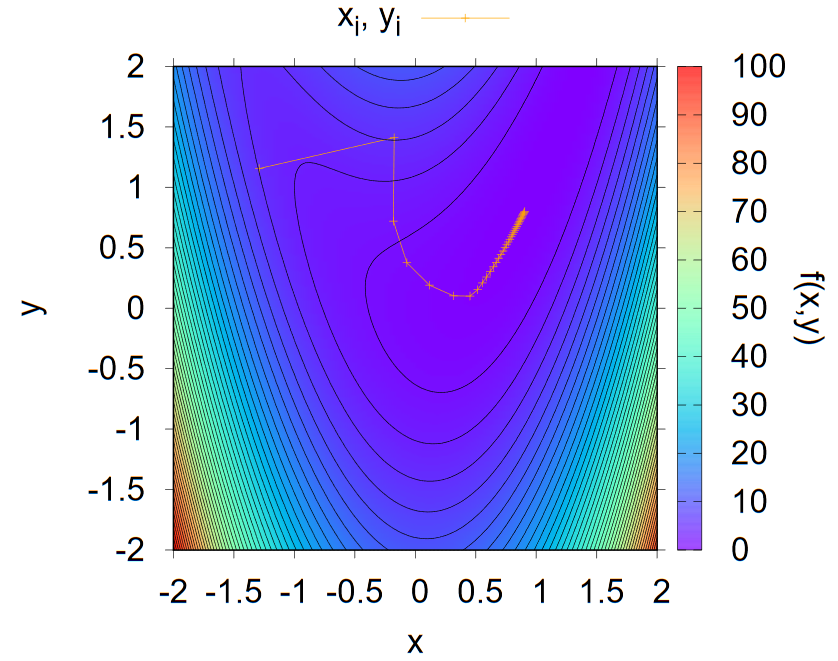
\includegraphics[height=0.41\linewidth]{min1.png}
	\caption{Położenia kolejnych przybliżeń minimum funkcji $ f(x, y) $ w poszczególnych iteracjach dla $\epsilon = 10^{-2} $. W tle: kontury oraz mapa wartości funkcji $ f(x, y) $. Program wykonał 37 iteracji.}
	\label{pierwszy} 
	\end{center}
\end{figure}
\begin{figure}[h!]
	\begin{center}
	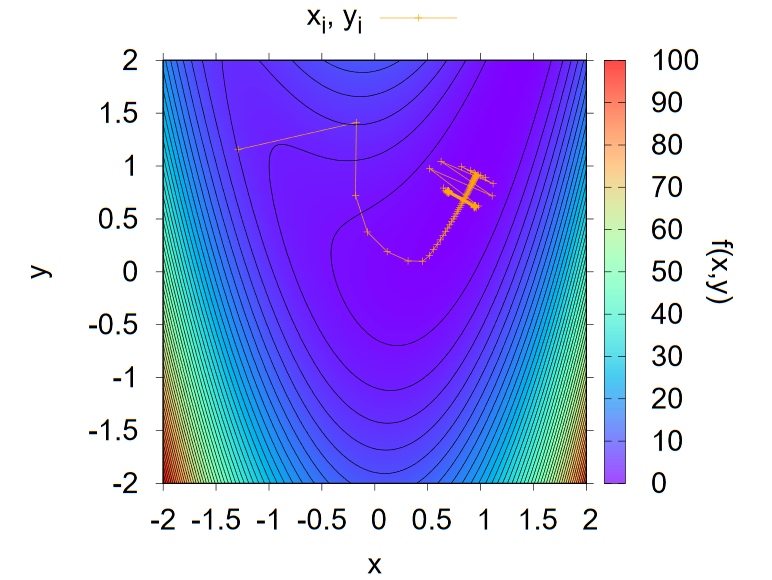
\includegraphics[height=0.41\linewidth]{min2.png}
	\caption{Położenia kolejnych przybliżeń minimum funkcji $ f(x, y) $ w poszczególnych iteracjach dla $\epsilon = 10^{-3} $. W tle: kontury oraz mapa wartości funkcji $ f(x, y) $. Program wykonał 1000 iteracji.}
	\label{drugi} 
\end{center}
\end{figure}

\newpage
\section{Wnioski}


\end{document}